\section{Quellencodierung}
Die Entropiecodierung hat das Ziel, Redundanz einer gedächnisfreien Quelle zu reduzieren. \script{209}
\begin{enumerate}[nosep]
	\item Fixed-Length
	\item Variable-Length
	\item Präfixfrei
	\item Eindeutig decodierbar
	\item unmittelbar decodierbar
\end{enumerate}

\subsection{Redundanz und Effizienz}\label{redundanz}
\script{211} Eine DMS (Gedächnisfreie Quelle) dessen Symbolwerte $x_i$ mit Wahr.keit $P(x_i)$ auftreten, und auf ein Codewort $c$ mit Länge $n$ und Anzahl Symbole $m$ gemappt werden. Effizient ist die Codierung, wenn die \textbf{mittlere Codelänge} $L$ möglichst klein wird d.h. häufig vorkommende Codeworte sollen kurz sein. Die Entropie $H(X)$ (siehe Kapitel \ref{entropie}) muss kleiner sein als $L$!
\[
L = \sum_{i=1}^{m}P(x_i)n_i \ge H(X)
\]

\noindent\textbf{Redudanz} $R$ (in bit/Symbol) berechnt sich pro Symbol wie folgt:
\[
R = L - H(X)
\]
\textbf{Achtung:} Wenn $32\times32$ Pixel für ein Icon verwendet werden, berechnet sich die totale entfernte Redudanz mit $R = 32\cdot32(L_1 - L_2)$, weil pro Symbol Redundanz entfernt wird.~\\~\\


\noindent Die \textbf{Effizienz} für die Quellencodierung berechnet sich wie folgt:
\[
\eta = \frac{H(X)}{L} \le 1
\]

\subsection{Codierung}
\subsubsection{Shannon-Fano}\script{212}
Die Shannon-Fano Codierung ist Präfix-frei und letzter Teilungsschritt liefert immer gerade Anzahl Codewörter.
\begin{enumerate}[nosep]
	\item Symoble nach \textbf{absteigender} Wahr.keit anordnen
	\item Trennung in \textbf{2 Teilmengen} mit möglichst gleicher Wahr.keit
	\item \textbf{Obere} Teilmenge Symbol $0$, \textbf{untere} Teilmenge Symbol $1$ zuordnen
	\item Solange die Teilmengen weiter unterteilen werden können, fortfahren bei 2
\end{enumerate}
\begin{center}
	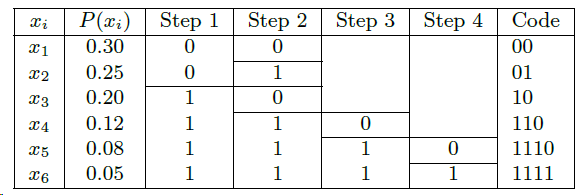
\includegraphics[width=\columnwidth]{Images/shannon-fano}
\end{center}

\subsubsection{Huffman}\script{213}
Huffman Codierung liefert die maximale Effizienz und haben keine reduntante Bits. Eine Eigenschaft von dieser Codierung ist, dass die längste Anzahl Bits immer gerade ist.
\begin{enumerate}[nosep]
	\item Symoble nach \textbf{absteigender} Wahr.keit anordnen
	\item Unterste beiden Symbole werden zu Symbolgruppe zusammengefasst
	\item Weiter bei 1, bis nurnoch zwei Symbolgruppen vorliegen
	\item Symbolegruppe mit höherer Wahr.keit wird $0$, die ander emit $1$ zugewiesen
	\item Letzter Reduktionsschritt rückgängig machen
	\item Weiter bei 4, bis keine Symbolgruppen mehr expandiert werden können
\end{enumerate}
\begin{center}
	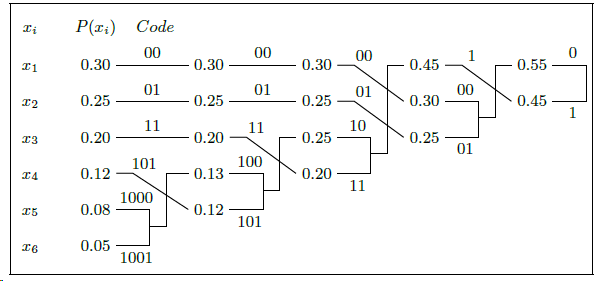
\includegraphics[width=\columnwidth]{Images/huffman}
\end{center}
Die mittlere Codewortlänge $L$ für die Effizient $\eta = \frac{H(X)}{L}$ ist:
\[
L = (0.3+0.25+0.2)\cdot2 + 0.12\cdot 3 + (0.8+0.05)\cdot 4 = 2.38
\]
